\chapter{Introduction} \label{introduction}
This chapter will introduce the problem that is addressed in this project. 
Previous similar projects will be investigated, and the value of this research will be presented.

\section{Background and Motivation}

Traditionally the thermal diffusivity, otherwise referred to as the $\alpha$-value, of timber is based simply on the EN 1995:1-2-2004\citep{Euro:2004}, further referred to as the Eurocode, or similar standards.
This research project will aim to obtain the thermal diffusivity of cross-laminated SA-Pine timber by further analysing data originally obtained by \citet{Westhuyzen:2020} for their study of the samples' charring rate.

The thermal diffusivity of timber is an unobservable quality that cannot be measured directly.
However, thermal diffusivity is directly related to thermal conductivity ($\kappa$) and can be calculated when thermal conductivity is known.
The majority of this report will therefore discuss the methods used to obtain the thermal conductivity or $\kappa$-values, and the diffusivity will be calculated when interpreting the results.

Conductivity can be related to measurements of temperature and time through differential models. 
When heat conduction is calculated using finite element methods, the process is usually simplified to a linear problem \citep{Fish:2007}. 
Due to the changes in thermal conductivity of timber with temperature, as can be seen in EN 1995:1-2-2004 (page 49) and Figure \ref{euroK}, the conductivity cannot be linearly modelled.
The problem therefore lends itself to being analysed by inversion techniques. 
This approach will allow us to obtain information about the conductivity based on the combined information assumed prior to measuring, further referred to as the prior, and the measured data. 
Statistical inversion delivers a probability distribution, thereby providing a collection of conductivity estimates and their corresponding probabilities.
The approach taken in this report is unique due to the nature of data used, as the main purpose of this data's collection was to determine char rates and not thermal conductivity or diffusivity.
The difference in research goals means that more assumptions had to be made, in contrast to a experiment that intended to determine the thermal conductivity and would have controlled those variables.

Currently, the fire rating of specific timber samples is based on fire tests conducted in a furnace. 
The furnace is kept at increasing temperatures corresponding with the Standard or ISO 834 fire curve as specified in ISO 834 \citep{ISO:1999}.
This process becomes very costly if it must be repeated every time timber is used for construction, as timber has seen increased usage for multiple story construction projects over the past decades. 
This increase is partially due to the sustainability of timber as a construction material: not only is it renewable but it also has a small carbon footprint \citep{Salvadori:2017}.
Obtaining and standardising thermal diffusivity values for different species of timber will assist in more accurate modelling.
If modelling accuracy can be increased, the use of modelling to confirm fire tests or to replace small-scale fire tests will become more feasible.

	\begin{figure}
	\centering
	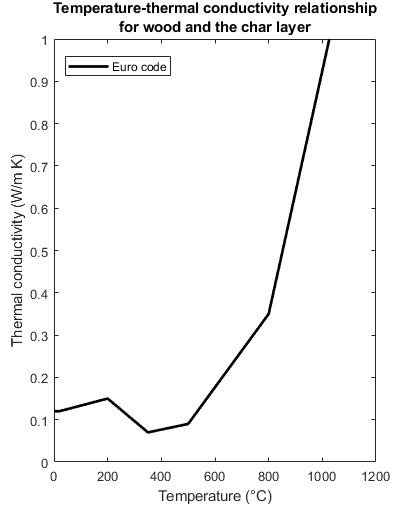
\includegraphics[width = 0.5\linewidth]{figures/Eurok.png}
	\caption{Standard temperature-thermal conductivity relationship for timber from \citep{Euro:2004}}
	\label{kvalue_fig}
	\end{figure}
	
	

\section{Aim and objectives}
During the course of the project, the student will aim to meet the following objectives:
\begin{enumerate}
 \item Modify a time-dependant heat transfer Finite Element Model implemented in Matlab into an accurate and effective function;
 \item Compare the model to the measured data;
 \item Solve for the thermal diffusivity using Bayesian Inversion using the following methods:
 	\begin{enumerate}
 		\item Maximum a Posteriori
 		\item Markov-chain Monte Carlo 	
 	\end{enumerate}
\end{enumerate}


\section{Literature study}\label{litstudy}
\iffalse
can be a bit longer: a) where does EC get its values from? is it relevant to SA? does SA have a timber code that includes our own values?  b) other problems (not necessarily fire) where material properties were determined using MCMC (there are thousands)
\fi
	
	In their article \textit{Simple Method to Determine the Diffusivity of Green Wood}, \citet{bioresource:2020}  determine the global diffusivity of a Douglas fir green log using inverse identification methods. 
	%In their experiment they also used thermocouples but only 3 at each end.  
	Their experiment involved submerging the log with K-type thermocouples attached at each end in a boiler filled with water at 60\textdegree C.
	The thermocouples were specifically placed to improve the accuracy of the diffusivity ratio calculation.
	The finite element model constructed for their calculations used linear interpolation with four-node quadrangle elements.
	An analytical model was also constructed using the heat conduction and diffusion equations.
	The thermal diffusivity was calculated by minimising the root mean square error between the slope of the measured data and the finite element model.
	This research intended to assist the peeling industry in making the pretreatment process more cost-effective.
	The method proved to be effective at determining the thermal diffusivity of green Douglas fir logs, as the $\kappa$-values obtained were comparable to those from literature.
	A crucial difference remains as the temperatures at which these experiments were conducted as well as the final usage of the data differ greatly.

%	A similar method of analysis was used by \cite{DeKoker:2021} in their article \textit{Assessment of ice impact load threshold exceedance in the propulsion shaft of an ice-faring vessel via Bayesian inversion}. 
%	Bayesian inversion is used to determine the impact of ice on the propellers from the measurements taken at a specified distance from the propeller. (TODO)

\citeauthor{Wagner:2021} wrote an article in March 2021 where Bayesian model inversion was used with stochastic spectral embedding.
Spectral embedding, or spectral likelihood expansion, was used to solve for the likelihood function in such a way that sampling is not necessary.
Similarly to this report, the research of \citet{Wagner:2021} involved the creation and use of a Bayesian model to solve a heat diffusion problem.
The likelihood function used for this analysis was similar to the likelihood function explained later in the report.
The focus of the article was to determine the accuracy of stochastic spectral likelihood embedding, stochastic spectral embedding and spectral likelihood functions to calculate the thermal diffusivity.
A Markov chain Monte Carlo analysis was done to compare to values from other methods.
Although the Markov chain Monte Carlo method was not discussed in detail in the article, the usage of Bayesian modelling to create a likelihood function that the MCMC analysis could be done on is similar to the process followed throughout this project.

%\citet{Thi:2016}
During the World Conference on Timber Engineering, \citet{Thi:2016} presented a paper regarding the mathematical modelling of timber in fire. 
In their model they considered the accounted for heat transfer through thermal conduction, convection and radiation similar to what was done in the model created for this project.
Their model was created in Abaqus and compared the model using different thermal conductivities and specific heat values.
The main goal of this model was to determine the change of the cross-section of timber due to charring, to achieve this the model had to be constructed in three-dimensions.
Their research proves that numerical modelling can be used to accurately predict the charring of timber and the change in cross section.
The effect of different thermal conductivity values on the resulting temperature curves produced by their model is also clear in their results.


The current Eurocode thermal $\kappa$-values were based on a study by \citet{Koning:1999}.
The most significant change in the $\kappa$-values obtained by \citeauthor{Koning:1999} compared to those of previous studies occurred after 350\textdegree C. 
This significant jump in the thermal conductivity is because the values modelled by the authors also encompassed the additional heat transfer due to cracks in the charred layer.
This cracking effect was assumed to occur at around 500\textdegree C.
These values were solved for using the computer program TEMPCALC.
TEMPCALC is based on a two-dimensional finite element model that solves for the temperature dependant thermal properties using the differential heat transfer equations.
The values obtained by \citeauthor{Koning:1999} are shown in Table \ref{tablekoning}.

\begin{table} 
	\caption{$\kappa$-values at different temperatures obtained by \citeauthor{Koning:1999}}
	\label{tablekoning}
	\begin{tabular}{ r r }
	\toprule
	Temperature & Conductivity\\
	{\textdegree}C & W/(m\ K)\\
	\midrule
	0&0.12\\
	200&0.15\\
	350&0.07\\
	500&0.09\\
	800&0.35\\
	1200&1.50\\
	\bottomrule
	\end{tabular}
\end{table}

